% ============================================================
%  CHAPITRE 4 — SPRINT 2 : GESTION DES DONNÉES DE RÉFÉRENCE
% ============================================================
\chapter{Sprint 2 : Gestion des Données de Référence}

\chapintro{Ce sprint met en place les données fondamentales~: tenants, garages,
personnel, véhicules et inventaire des pièces détachées.}

\section{Introduction}

Les données de référence constituent le socle métier sans lequel aucune opération
n'est possible~: un garage doit exister pour accueillir des rendez-vous, un véhicule
doit être enregistré pour soumettre des symptômes, et les pièces détachées doivent
être référencées pour être incluses dans les factures.

\section{Identification du Backlog Sprint 2}

\begin{table}[H]
\centering
\caption{Backlog Sprint 2 --- Données de Référence}
\label{tab:backlog-s2}
\begin{tabularx}{\textwidth}{|l|X|l|c|}
\hline
\rowcolor{gray!20}
\textbf{ID} & \textbf{User Story} & \textbf{Priorité} & \textbf{SP} \\
\hline
US05 & SuperAdmin~: créer et gérer les tenants & \prio{H} & 3 \\[3pt]\hline
US06 & AdminEntreprise~: créer et gérer des garages & \prio{H} & 5 \\[3pt]\hline
US07 & AdminEntreprise~: gérer le personnel (chefs, mécaniciens) & \prio{H} & 5 \\[3pt]\hline
US08 & Client~: enregistrer ses véhicules & \prio{H} & 3 \\[3pt]\hline
US09 & AdminEntreprise~: gérer l'inventaire des pièces détachées & \prio{M} & 5 \\[3pt]\hline
\multicolumn{3}{|r|}{\textbf{Total Sprint 2}} & \textbf{21 SP} \\
\hline
\end{tabularx}
\end{table}

\noindent\textbf{Tâches techniques~:}
\begin{enumerate}[noitemsep]
  \item Entités de domaine~: \texttt{Garage}, \texttt{Vehicle}, \texttt{SparePart}.
  \item Commandes CQRS~: \texttt{CreateGarageCommand}, \texttt{CreateVehicleCommand},
    \texttt{CreateSparePartCommand}, \texttt{CreateStaffCommand}.
  \item Migrations EF Core pour les nouvelles tables.
  \item Contrôleurs REST~: \texttt{GaragesController}, \texttt{VehiclesController},
    \texttt{SparePartsController}.
  \item Politiques d'autorisation par rôle (\texttt{[Authorize(Roles = ...)]}).
  \item Tableau de bord administrateur Angular.
\end{enumerate}

\section{Conception}

\subsection{Diagramme de cas d'utilisation --- Sprint 2}

\begin{figure}[H]
\centering
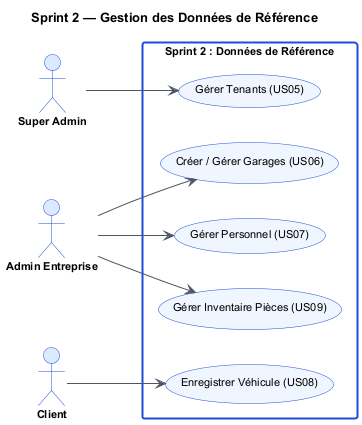
\includegraphics[width=0.85\textwidth]{diagrams/uc_s2.png}
\caption{Diagramme de cas d'utilisation --- Sprint 2}
\label{fig:uc-s2}
\end{figure}

\subsection{Diagramme de classes --- Sprint 2}

\begin{figure}[H]
\centering
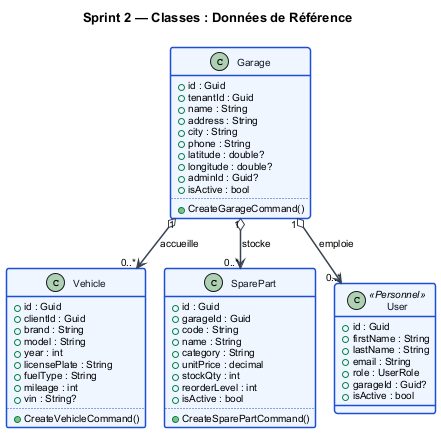
\includegraphics[width=\textwidth,height=0.62\textheight,keepaspectratio]{diagrams/class_s2.png}
\caption{Diagramme de classes --- Sprint 2 (Données de Référence)}
\label{fig:class-s2}
\end{figure}

\subsection{Diagramme de séquence}

\subsubsection*{SC3 --- Création d'un Garage (US06) : fonctionnalité principale}

\noindent L'admin entreprise crée un nouveau garage après vérification de l'existence
du tenant.

\begin{sidewaysfigure}[p]
\centering
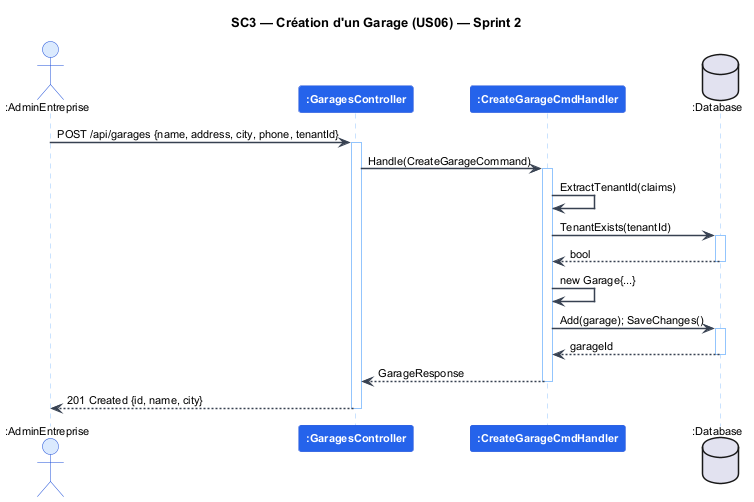
\includegraphics[width=0.92\textheight,keepaspectratio]{diagrams/seq_s2_garage.png}
\caption{Diagramme de séquence SC3 --- Création d'un Garage}
\label{fig:seq-s2-garage}
\end{sidewaysfigure}

\section{Conclusion}

Le Sprint 2 a mis en place les données de référence essentielles. Les politiques
d'autorisation par rôle ont été appliquées de façon granulaire~: seul un
\texttt{AdminEntreprise} peut créer un garage, et un \texttt{Client} ne gère que
ses propres véhicules.
